\chapter{Десорбция дейтерия из вольфрама при импульсном лазерном нагреве}\label{ch:ch4}

\section{Валидация}\label{sec:ch4/sec1}

Исходные данные, расчетные коды и результаты сравнения представлены в открытом (\todo{необходимо сделать архив zenodo}) \href{https://github.com/KulaginVladimir/LID-validation}{доступе}.

\subsection{Детали эксперимента по лазерно-индуцированной десорбции дейтерия из вольфрамовых пленок}\label{subsec:ch4/sec1/subsec1}

Эксперименты для проверки корректности модели ЛИД проводились на базе физико-технического института им. А. Ф. Иоффе. В экспериментах использовались пленки со-осаждения вольфрама и дейтерия. Пленки были нанесены на медные подложки ($20 \times 20 \times \SI{3}{\milli\metre}$) методом импульсного лазерного осаждения в атмосфере дейтерия (давление \SI{30}{\pascal}) с плазменным ассистированием при частоте \SI{13.56}{\mega\hertz}. Для осаждения плёнок вольфрама использовался твердотельный лазер Nd:YAG с длиной волны \SI{1064}{\nano\meter}, энергией в импульсе \SI{1.3}{\joule}, длительностью импульса \SI{12}{\nano\second} и частотой следования импульсов \SI{10}{\hertz}. Лазерное излучение фокусировалось на вольфрамовой мишени для обеспечения плотности энергии $\approx\SI{25}{\joule\per\centi\meter\squared}$. Осаждение проводилось в течение 15 минут при водяном (\SI{18}{\degreeCelsius}) охлаждении держателя. Толщина осажденных пленок составила $\approx\SI{1}{\micro\metre}$.

Полученные образцы укладывались на медное основание ($100 \times 80 \times \SI{3}{\milli\metre}$). Для обеспечения лучшего теплоотвода во время ЛИД между медным основанием и образцами устанавливались индиевые прокладки. Композитная мишень фиксировалась медной рамкой с окошками, как показано на рисунке~\cref{fig:ch4/LID_target}. Образцы облучались лазерными импульсами с длительностью \SI{250}{\micro\second} и \SI{1}{\milli\second} (оптоволоконная лазерная система, IPG YLR-2000, \SI{1070}{\nano\metre}). Полная энергия лазерных импульсов варьировалась в диапазоне от \SI{0.124}{\joule} до \SI{0.351}{\joule} и от \SI{0.255}{\joule} до \SI{1.003}{\joule} для микросекундной и миллисекундой длительности импульса, соответственно. Облучение поверхности образцов при максимальной энергии из диапазонов не приводило к изменениям поверхности, что позволило

\begin{figure}[ht]
    \centerfloat{
        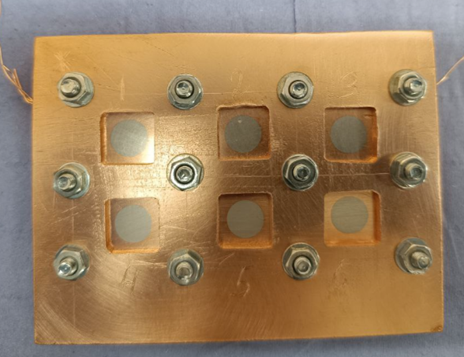
\includegraphics[scale=0.8]{LID_target.png}
    }
    \caption{Вид образцов с пленками вольфрама, расположенных на медном основании. Серые области "--- вольфрам-дейтериевые пленки}\label{fig:ch4/LID_target}
\end{figure}

Пространственный профиль плотности энергии измерялся лазерным анализатором SP620U OPHIR-SPIRICON. Полученный профиль представлен на рисунке~\cref{fig:ch4/laser_spatial_distr} и соответствует распределению Гаусса с усредненным значением полной ширины на уровне $1/e^2$ равным \SI{1}{\milli\metre}.

\begin{figure}[ht]
    \centerfloat{
        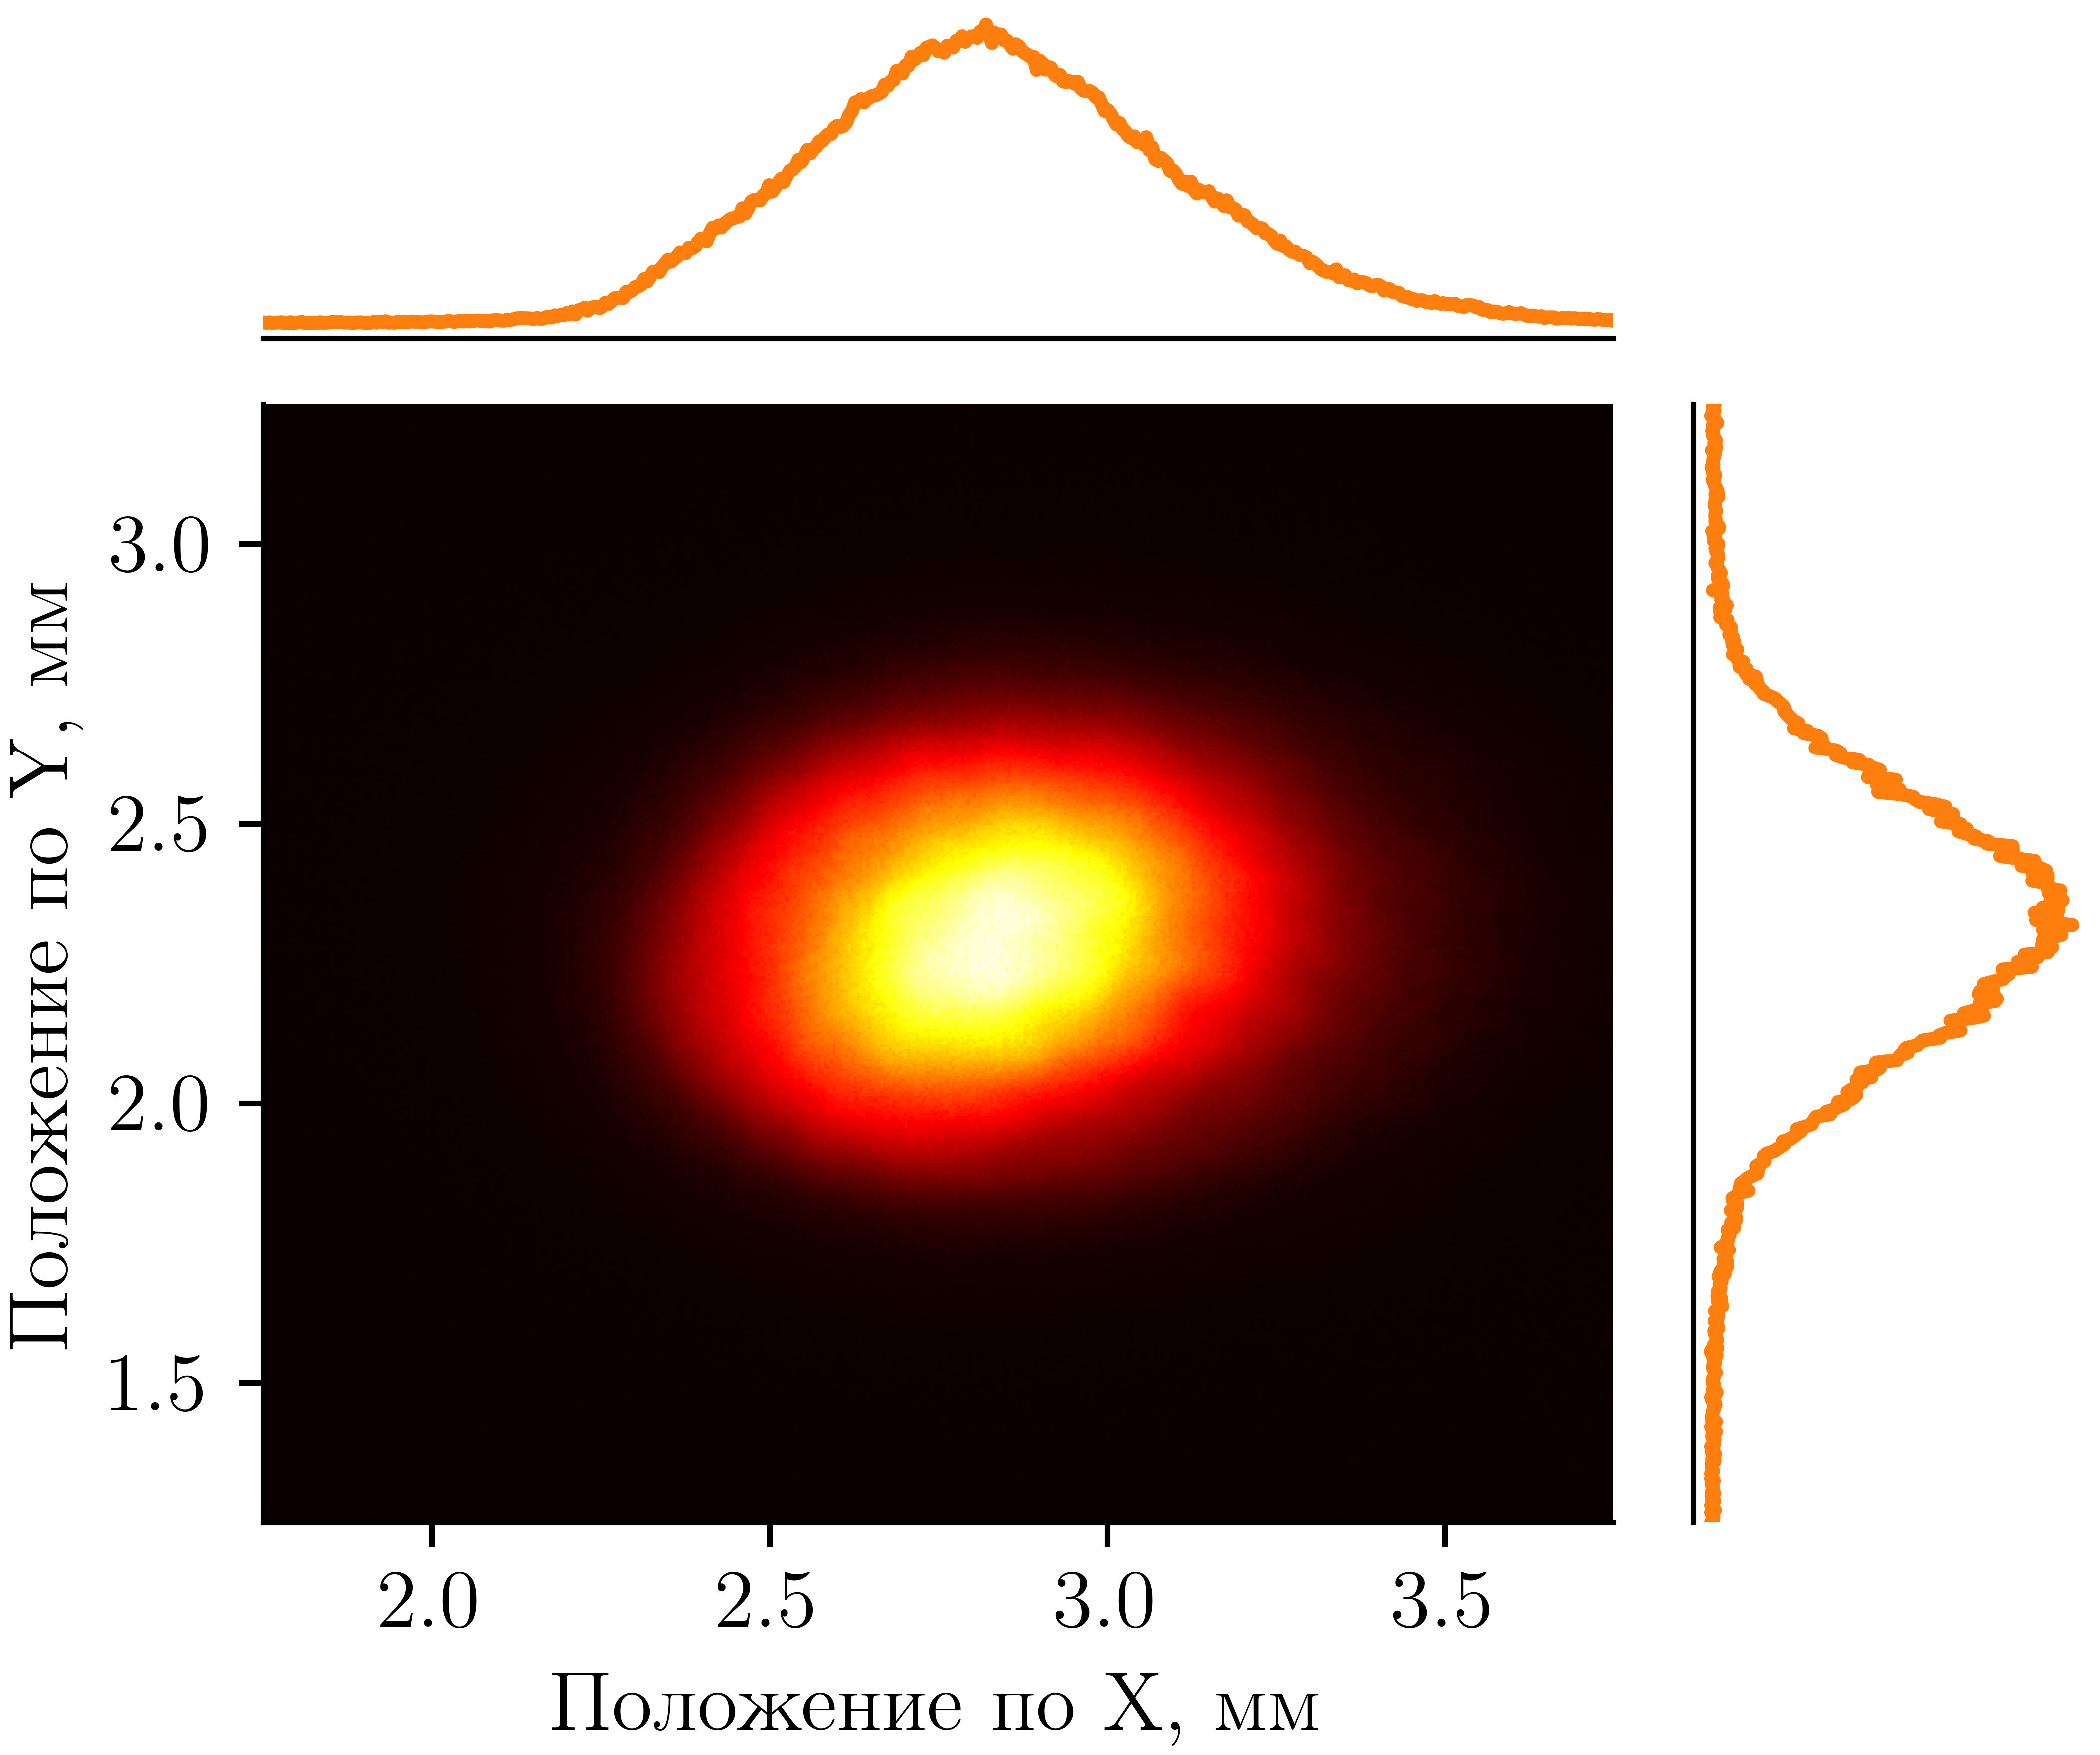
\includegraphics[scale=1]{laser_spatial_distr.png}
    }
    \caption{Пространственное распределение плотности энергии в лазерном импульсе длительностью \SI{1}{\milli\second}}\label{fig:ch4/laser_spatial_distr}
\end{figure}

\fixme{Временные профили лазерного импульса измерялись кремниевым фотодиодом ФДУК-200 в фотогальваническом режиме. Временной профиль имел трапециевидною форму с экспоненциально растущим/затухающим фронтами. Пример временного профиля длительностью 1 мс приведен на рисунке 3.} Экспериментальный стенд для исследования ЛИД (см. рисунок~\ref{fig:ch4/LID_scheme}) включал в себя оптическую схему на основе двухлинзовой фокусирующей системы Галилея, систему перемещения лазерного луча по поверхности и вакуумный объём ($\approx\SI{70}{\liter}$). 
\begin{figure}[ht]
    \centerfloat{
        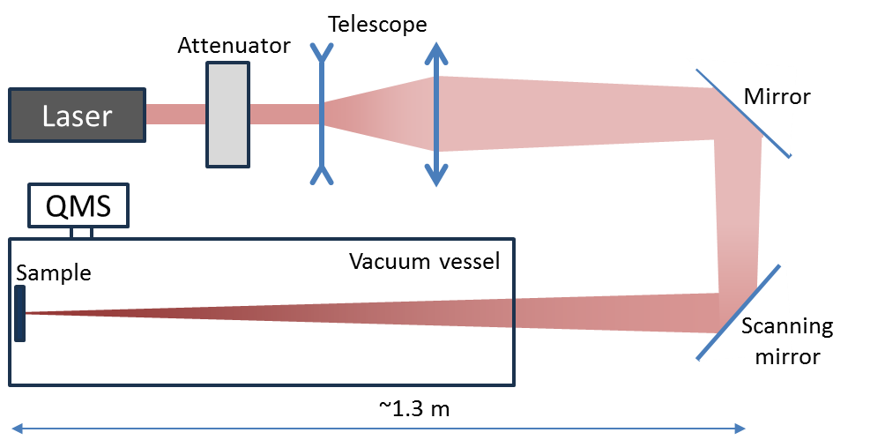
\includegraphics[scale=0.6]{LID_optic_scheme.png}
    }
    \caption{Схема установки для проведения измерений ЛИД~\cite{Medvedev2024}}\label{fig:ch4/LID_scheme}
\end{figure}
Вакуумный объём откачивался турбомолекулярным насосом (Turbovac 90i, Leybold) до базового уровня давления \SI{8e-5}{\pascal}. Для каждой энергии лазерного пучка проводилась серия импульсов с частотой \SI{0.1}{\hertz}. Регистрация сигнала 2, 3, 4 масс проводилась квадрупольным масс-спектрометром (Extorr XT300M). \fixme{Пример временной зависимости сигналов 3 и 4 масс представлен на рисунке 4}. Масс-спектрометр калибровался по постоянному потоку дейтериевой течи с уровнем потока \SI{e-6}{\metre\cubed\pascal\per\second}. После серии импульсов энергия лазерного пучка и область облучения поверхности в пределах одного образца менялись. Смещение лазерного пятна происходило на такое расстояние, чтобы избежать влияния предыдущих импульсов на результаты измерений последующих. Для упрощения сравнения результатов численного моделирования с экспериментом из каждой серии импульсов при различных энергиях пучка использовались только первые выстрелы. Откалиброванный сигнал от первого выстрела интегрировался по времени для определения полного числа десорбированных атомов дейтерия. \fixme{Пример откалиброванной временной зависимости потока дейтерия представлен на рисунке 5}.

\subsection{Определение параметров центров захвата дейтерия}\label{subsec:ch4/sec1/subsec2}

Одними из неизвестных параметров в задаче ЛИД дейтерия из со-осажденных пленок вольфрама являются параметры центров захвата дейтерия. Для определения этих параметров был проведен ТДС анализ аналогичных образцов с пленками толщиной \SI{0.5}{\micro\metre}. ТДС-анализ был проведен на сверхвысоковакуумном стенде \thesisOrganizationShort \ (кафедра №21), схема которого приведена на рисунке~\cref{fig:ch4/TDS_setup}. 

\fixme{Сверхвысоковакуумный термодесорбционный стенд создан для изучения захвата водорода в образцы, облученные в различных плазменных установках вне камеры, не обладающих возможности проведения ТДС анализа без переноса по атмосфере~\cite{Rusinov2009}. Для повышения эффективности работы стенд был сконструирован так, чтобы минимизировать время замены образцов, а Для повышения эффективности работы стенд был сконструирован так, чтобы минимизировать время замены образцов, а также свести к минимуму газовыделение с внутренних конструкционных элементов в ходе ТДС измерений Основная камера представляет собой цилиндр диаметром 150 мм и
длиной 230 мм. Высокий вакуум (< 2×10−9 мбар) в камере обеспечивается турбомолекулярным насосом с безмасляной форвакуумной откачкой.} 

\fixme{На случай длительных перерывов в измерениях дополнительно установлен магниторазрядный насос, который отсекается в ходе ТДС измерений. В центре камеры располагается ленточный нагреватель, изготовленный из вольфрама (толщина 25 мкм), который закрепляется на двух охлаждаемых водой токовводах (рис.2.11). При замене образцов развакуумируется только шлюзовая камера, отделенная проходным клапаном и имеющая собственную независимую откачку. Перемещение образца в камеру измерений
осуществляется с помощью сильфонного ввода движения (ход 250 мм). Образец подвешивается к вводу движения на приваренной к нему вольфрамрениевой термопаре, которой измеряется и температура образца. Для фиксации более "тяжелых" образцов изготавливается и предварительно обезгаживается дополнительный держатель из вольфрама или молибдена. Между камерой загрузки образцов и камерой проведения ТДС устанавливается дополнительный запирающий элемент. При достижении образцом зоны нагрева отверстие в этом элементе перекрывается. При этом сводится к минимуму поток атмосферных газов в камеру измерения. Такая конструкция позволила сократить время замены образцов. Для достижения максимальной температуры в ряде экспериментов использовались дополнительные тепловые экраны из вольфрамовой фольги, окружающие область нагрева. Это позволило для небольших (6×6 мм2) образцов из вольфрамовой фольги достичь температуру 2550 К, что недоступно на большинстве установок для термодесорбционных измерений. Столь большая температура обычно не требуется, но ее достижение позволило зарегистрировать высокотемпературную десорбцию гелия из вольфрама. Линейный нагрев, как и в случае установки Медион, обеспечивается системой ПИД регуляции [169]. Отклонение от линейности роста температуры наблюдалось только на начальной стадии нагрева, до температуры ~ 380 K.} 

\begin{figure}[ht]
    \centerfloat{
        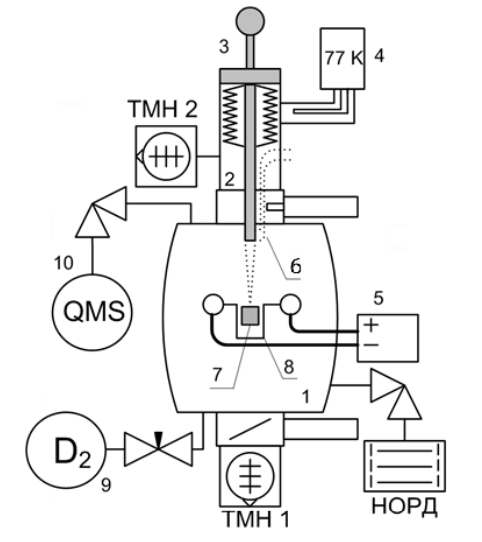
\includegraphics[scale=0.75]{TDS_setup.png}
    }
    \caption{Принципиальная схема ТДС-стенда: 1 "--- камера измерений, 2 "--- шлюзовая камера, 3 "--- ввод движения, 4 "--- азотная ловушка, 5 "--- блок питания нагрева, 6 "--- термопара, 7 "--- образец, 8 "--- вольфрамовый нагреватель, 9 "--- резервуар с дейтерием, 10 "--- квадрупольный масс-спектрометр~\cite{Rusinov2009}}\label{fig:ch4/TDS_setup}
\end{figure}

\subsection{Расчетная модель}\label{subsec:ch4/sec1/subsec3}
\subsection{Сравнение результатов моделирования и эксперимента}\label{subsec:ch4/sec1/subsec4}

\section{Анализ состава потока десорбированных частиц}\label{sec:ch4/sec2}
\subsection{Постановка задачи}\label{subsec:ch4/seс2/subsec1}
\subsection{Аналитический анализ}\label{subsec:ch4/seс2/subsec2}
\subsection{Результаты численного моделирования}\label{subsec:ch4/seс2/subsec3}

\section{Анализ влияния параметров материала на выход дейтерия}\label{sec:ch4/seс3}
\subsection{Постановка задачи}\label{subsec:ch4/seс3/subsec1}
\subsection{Влияние теплопроводности материала}\label{subsec:ch4/seс3/subsec2}
\subsection{Влияние параметров дефектов в вольфраме}\label{subsec:ch4/seс3/subsec3}
\subsection{Влияние градиента температур}\label{subsec:ch4/seс3/subsec4}
\subsection{Режимы десорбции во время лазерно-индуцированной десорбции}\label{sec:ch4/seс4/subsec5}

\section{Выводы к Главе~\ref{ch:ch4}}

\clearpage
